\chapter{Imitando a Lope de Vega} \label{chapter6}
Abordamos ahora el problema que nos hemos propuesto: entrenar una red para generar texto al estilo de Lope de Vega utilizando GPT. Con este fin, se ha desarrollado una implementación completa de la familia GPT utilizando la librería \textit{Pytorch}. Esta implementación, que utiliza estrategias como la aceleración de \textit{hardware} o la precisión mixta para aumentar la eficiencia, puede encontrarse en el \cref{appendixA}, junto al código utilizado para generar los resultados introducidos en esta sección. Todos los resultados pueden reproducirse utilizando el código y los modelos entrenados, que se encuentran disponibles en un repositorio de acceso público \cite{githubrepo}.

Además, se ha creado \textit{ex profeso} un conjunto de datos con alrededor de 51.000 líneas de texto plano, provenientes de distintas obras dramáticas y abierto al público, a fin de que sea posible replicar nuestros resultados \cite{lopedataset}.

A fin de homogeneizar el texto y facilitar el entrenamiento se han mantenido únicamente los diálogos eliminando acotaciones, notas y textos accesorios, como los prólogos. También se han unificado los símbolos ortográficos para no ampliar el tamaño del vocabulario sin necesidad.

El conjunto de datos se ha dividido en un conjunto de entrenamiento con el \( 90\% \) de los caracteres y un conjunto de validación con el \( 10\% \) restante. Dado que no se va a evaluar el rendimiento del modelo posteriormente y el tamaño del conjunto de datos es limitado, se prescinde de un conjunto de prueba.

\begin{algorithm}[tb]
  \SetAlgoLined
  \KwData{$\Set{x_n}_{n = 0}^N$, con $x_n \in \mathbb{V}^*$, conjunto de entrenamiento}
  \mydata{$\theta \in \Theta$, parámetros iniciales}
  \KwHyper{$\Lambda$, parámetros de Adam (\cref{algo:adam})}
  \mydata{$N_\text{iter}$, número de iteraciones}
  \mydata{$N_\text{lote}$, tamaño de minilote}

  \For{$t = 1, …, N_\text{iter}$} {
    Muestrear un minilote: $\Set{x_{1}, …, x_{N_\text{lote}}}$ \;
    para $n = 1, …, N_\text{lote}$: $P(\theta)[n, :, :] \gets \texttt{GPT}(x_n \mid \theta)$ \;
    $L(\theta) = \sum_{n = 1}^{N_\text{lote}} \sum_{t = 1}^{|x_n| - 1} \log(P(\theta))[n, x_n[t + 1], t]$ \;
    $\theta \gets \texttt{Adam}(\theta, L; \Lambda)$ \;
  }
  \Return{$\theta$}

  \caption{Entrenamiento de GPT usando Adam \cite{phuong2022formal}}
  \label{algo:gpt_train}
\end{algorithm}

\section{Primera aproximación al problema}
A fin de poder comprobar el correcto funcionamiento del modelo y entrenarlo con facilidad, hemos realizado una primera aproximación al problema utilizando un modelo  GPT muy sencillo, formado por seis bloques de tipo decodificador con atención multicabezal con seis cabezales.

\subsection{Entrenamiento de la red}
\begin{figure}[tb]
    \centering
    \begin{subfigure}[b]{0.49\textwidth}
        \centering
        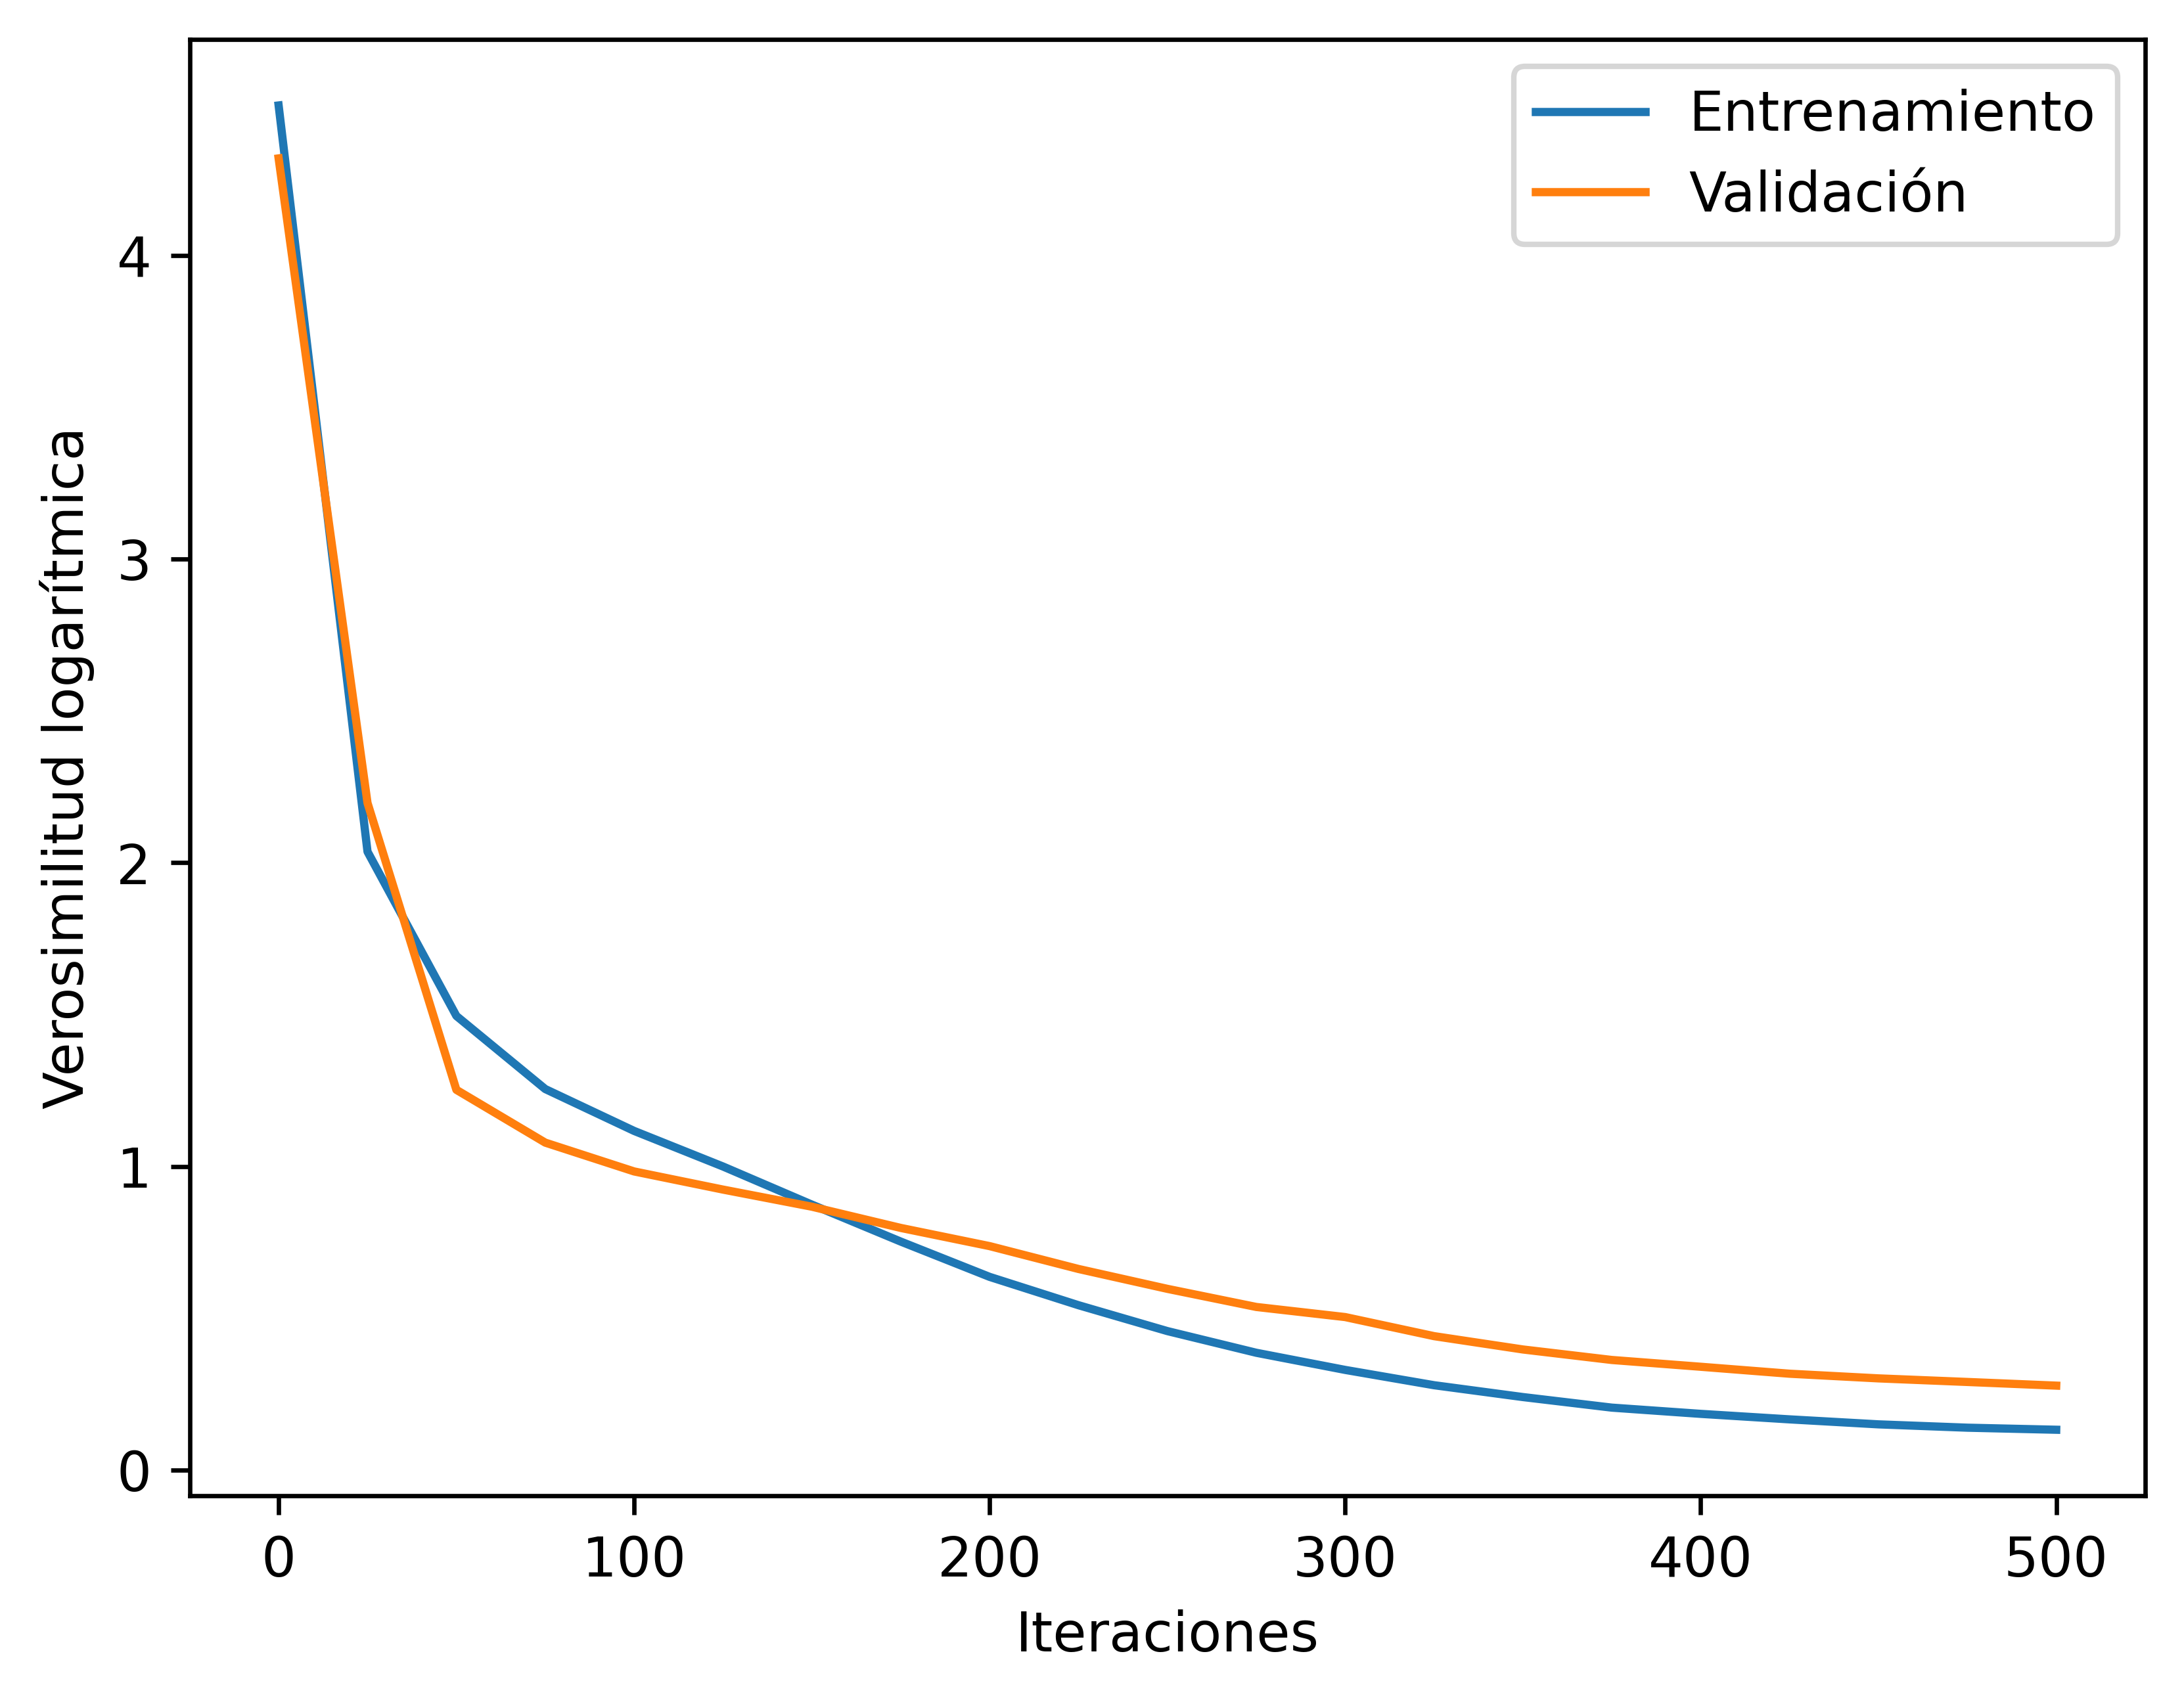
\includegraphics[width=\textwidth]{figures/chapter5/mini_loss.png}
        \caption{Entrenamiento de un modelo GPT mínimo}
        \label{fig:loss}
    \end{subfigure}
    \begin{subfigure}[b]{0.49\textwidth}
        \centering
        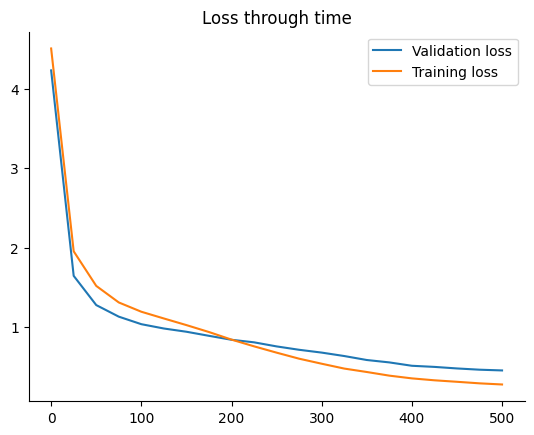
\includegraphics[width=\textwidth]{figures/chapter5/loss.png}
        \caption{Entrenamiento de GPT-2}
        \label{fig:loss_big}
    \end{subfigure}
    \caption{Pérdida promedio sobre el conjunto de entrenamiento y validación a lo largo del entrenamiento. La función de pérdida es la verosimilitud logarítimica (\cref{eq:unsupervised}). Nótese que los resultados de ambas gráficas no son comparables, pues utilizan \textit{tokenizaciones} distintas.}
\end{figure}

Se ha utilizado una tokenización a nivel de carácter, con una dimensión del espacio latente igual a 384 y longitud de contexto igual a 256. Aunque estos valores nos permiten utilizar un tamaño de minilote significativo (el modelo procesa 64 secuencias en paralelo), es de esperar que sean insuficientes para generar texto coherente. El modelo tiene un total de \( 10.65 \) millones de parámetros.

El modelo se ha entrenado de modo no supervisado utilizando el método de optimización \textit{Adam} (\( \epsilon = 10^{-3}, (\beta_1, \beta_2) = (0.99, 0.999) \)) durante un total de \( 500 \) iteraciones, utilizando el \cref{algo:gpt_train} y supervisando la convergencia sobre el conjunto de validación. El modelo converge adecuadamente, como muestra la \cref{fig:loss}.

Presentamos a continuación algunas muestras del texto generado por la red, utilizando el \cref{algo:gpt_inference}, que implementa la estrategia comentada en la \cref{sec:gen}. En el segundo caso, se utiliza el texto de estímulo para interactuar con la red: 

\noindent
\begin{table}[H]
  \centering
  \begin{tabular}{ l | l }
    \begin{Code}
    ¿Quién es este caballero
    Que te ha enseñado a ti?
    
    SANCHO:
    Y ¿Nuño? ¿Qué importa?
    Criados son de don Tello,

    A quien me mandaste hablar:
    ¡Mal haya, amén, el consejo!
    En este valle hay diez casas,
    Y no harán llenas mis cosas
    Que te han de costar la vida.
    
    SANCHO:
    Pues ¿de qué, señor?

    NUÑO:
    Por que una puerta ha sucedido,
    En que vos su voluntad
    Y aun aomaba primero,
    \end{Code}
    &
    \begin{Code}
    ESTEBAN:
    ¿Cómo?
    
    COMENDADOR:
    ¡Ah, señores!
    
    ESTEBAN:
    ¡A cosas tan cuerdas!

    COMENDADOR:
    ¡Perra de mi casa, ayer
    que la fe que habéis abrazar
    con la edad por ajenos!

    ÁLVARO:
    ¿Quién mató al comendador?
    
    COMENDADOR:
    Fuente Ovejuna lo hizo
    \end{Code}
  \end{tabular}
\end{table}

Como se puede ver, la red genera texto sintácticamente correcto y es capaz de replicar la estructura de diálogo, pero la mayor parte del texto generado carece de sentido. 

Los resultados son poco sorprendentes, toda vez que estamos intentando que un modelo  muy sencillo sin ninguna noción lingüística previa ``aprenda'' castellano y lo utilice para generar una estructura muy elaborada. 

\section{Afinando GPT-2 (\textit{finetuning})}
Los dos problemas anteriores (lo limitado del modelo y lo escaso del conjunto de entrenamiento) pueden aliviarse utilizando modelos pre-entrenados más grandes. Este modelo pre-entrenado se reentrena o \textit{afina} (\textit{fine-tune}) sobre nuestro conjunto de entrenamiento, para adaptarlo a la tarea específica. Este segundo entrenamiento no necesita ser tan intensivo como si entrenásemos la red desde cero, pues las representaciones iniciales de la red deberían ser cercanas a las finales, lo que permite ahorrar recursos computacionales y utilizar modelos de mucho mayor tamaño.

Partimos de una versión pre-entrenada sobre un corpus de texto de 11.5 GB, de diferentes fuentes \cite{gpt2trained} y entrenamos el modelo utilizando Adam durante 3.750 iteraciones. Hemos utilizado una tasa de aprendizaje \( \epsilon = 10^{-5} \) y se ha incluido abandono (\( p = 0.9 \)) para combatir el sobre-ajuste. Utilizamos una \textit{tokenización a nivel de byte por pares de byte}, ajustada al castellano.

Como es de esperar para un modelo tan complejo entrenado sobre un conjunto tan pequeño, el modelo muestra un claro sobre-ajuste aunque converge adecuadamente sobre el conjunto de validación.

Los resultados obtenidos son mucho más prometedores:
\noindent
\begin{table}[H]
  \centering
  \begin{tabular}{ l | l }
  \begin{Code}
    NARV:
    Hazte santo, y verás
    Que toda la gente pasa
    De su bien y su mal,
    Y que los reyes se engañan
    Si no reparan en esto,
    Que de una palabra se vale.
    
    ARR:
    Bien dices; que éste es el fin
    De mi vida, y que adoro
    En tan dulce estado,
    Y que el fin que veo me condena,
    Darle, el fin que quiero.    

    NARV:
    Escucha, Nuño, que me pesa
    De haber venido aquí,
    Nuño, tan abatido.

    NUÑO:
    Ya del estrecho celoso,
    Hija, el corazón ensancho.

    NARV:
    ¿Qué se ha hecho el pobre Sancho,
    Que solía ser mi esposo?
  \end{Code} 
  &
  \begin{Code}
    PAD:
    ¿Por qué razon
    Donde sola mi aficion
    Puede, como la espada
    Hace al desafío burlas?
    Porque guerra y casamiento
    Es un propio pensamiento,
    Todo es guerra, y si lo es todo,
    No sales del desafío.
    Si áun hay amor, yo me rindo;
    Si el de Aragon no manda,
    Padilla, yo me rindo á mí.
    
    ÁLV:
    ¿Qué mayor contento
    Que llegar como llego?
    
    PAD:
    Aquí me deja su alteza
    Á prevenir la jornada
    Que para Granada intenta,
    Porque pienso que ha de ser
    Luégo que la primavera
    Temple la furia á los rios,
    Seque la mojada tierra.  
  \end{Code}
\end{tabular}
\end{table}

El modelo tiene limitaciones: es propenso a cambiar bruscamente el tema de conversación y el sobre-ajuste provoca que reproduzca en ocasiones oraciones enteras del conjunto de entrenamiento. En cualquier caso, se trata de resultados excelentes dado lo reducido del conjunto de entrenamiento.

Si queremos generar texto de mayor calidad, el uso de una arquitectura tan escalable como los \textit{transformers} proporciona una hoja de ruta para generar mejores predicciones: aumentar el conjunto de datos y recurrir a arquitecturas de mayor escala (teniendo en cuenta que esto puede hacer necesaria una mayor regularización).

Para hacerse una idea de los costes computacionales implicados, afinar esta red sobre el conjunto de datos necesitó unas 10 horas en \textit{hardware} doméstico. GPT-2 no puede entrenarse de forma viable en este tipo de hardware, pues su entrenamiento necesita más de un mes en una tarjeta gráfica especializada. El afinamiento da acceso de una forma eficiente a estas arquitecturas, cuyo uso de otra manera requeriría costes inasumibles.

\section{Visualización del modelo}
Dadas matrices de consultas y claves \( Q = [q_1, …, q_{n_q}], K = [k_1, …, k_n] \) la entrada \( i, j \)-ésima de la \textit{matriz {de pesos de atención}}
\[
  \softmax \left( \frac{K^T Q}{\sqrt{d}} \right)
\] 
presente en el cálculo de la atención de producto normalizado se presta a ser interpretada como una medida de la similitud entre \( k_i \) y \( q_j \) e, indirectamente, como una medida de la similitud entre los elementos de la secuencia de entrada asociados a estas claves y consultas. Podemos utilizar esta propiedad para estudiar el comportamiento de los distintos cabezales de atención del modelo.

\begin{figure}[tb]
  \centering
  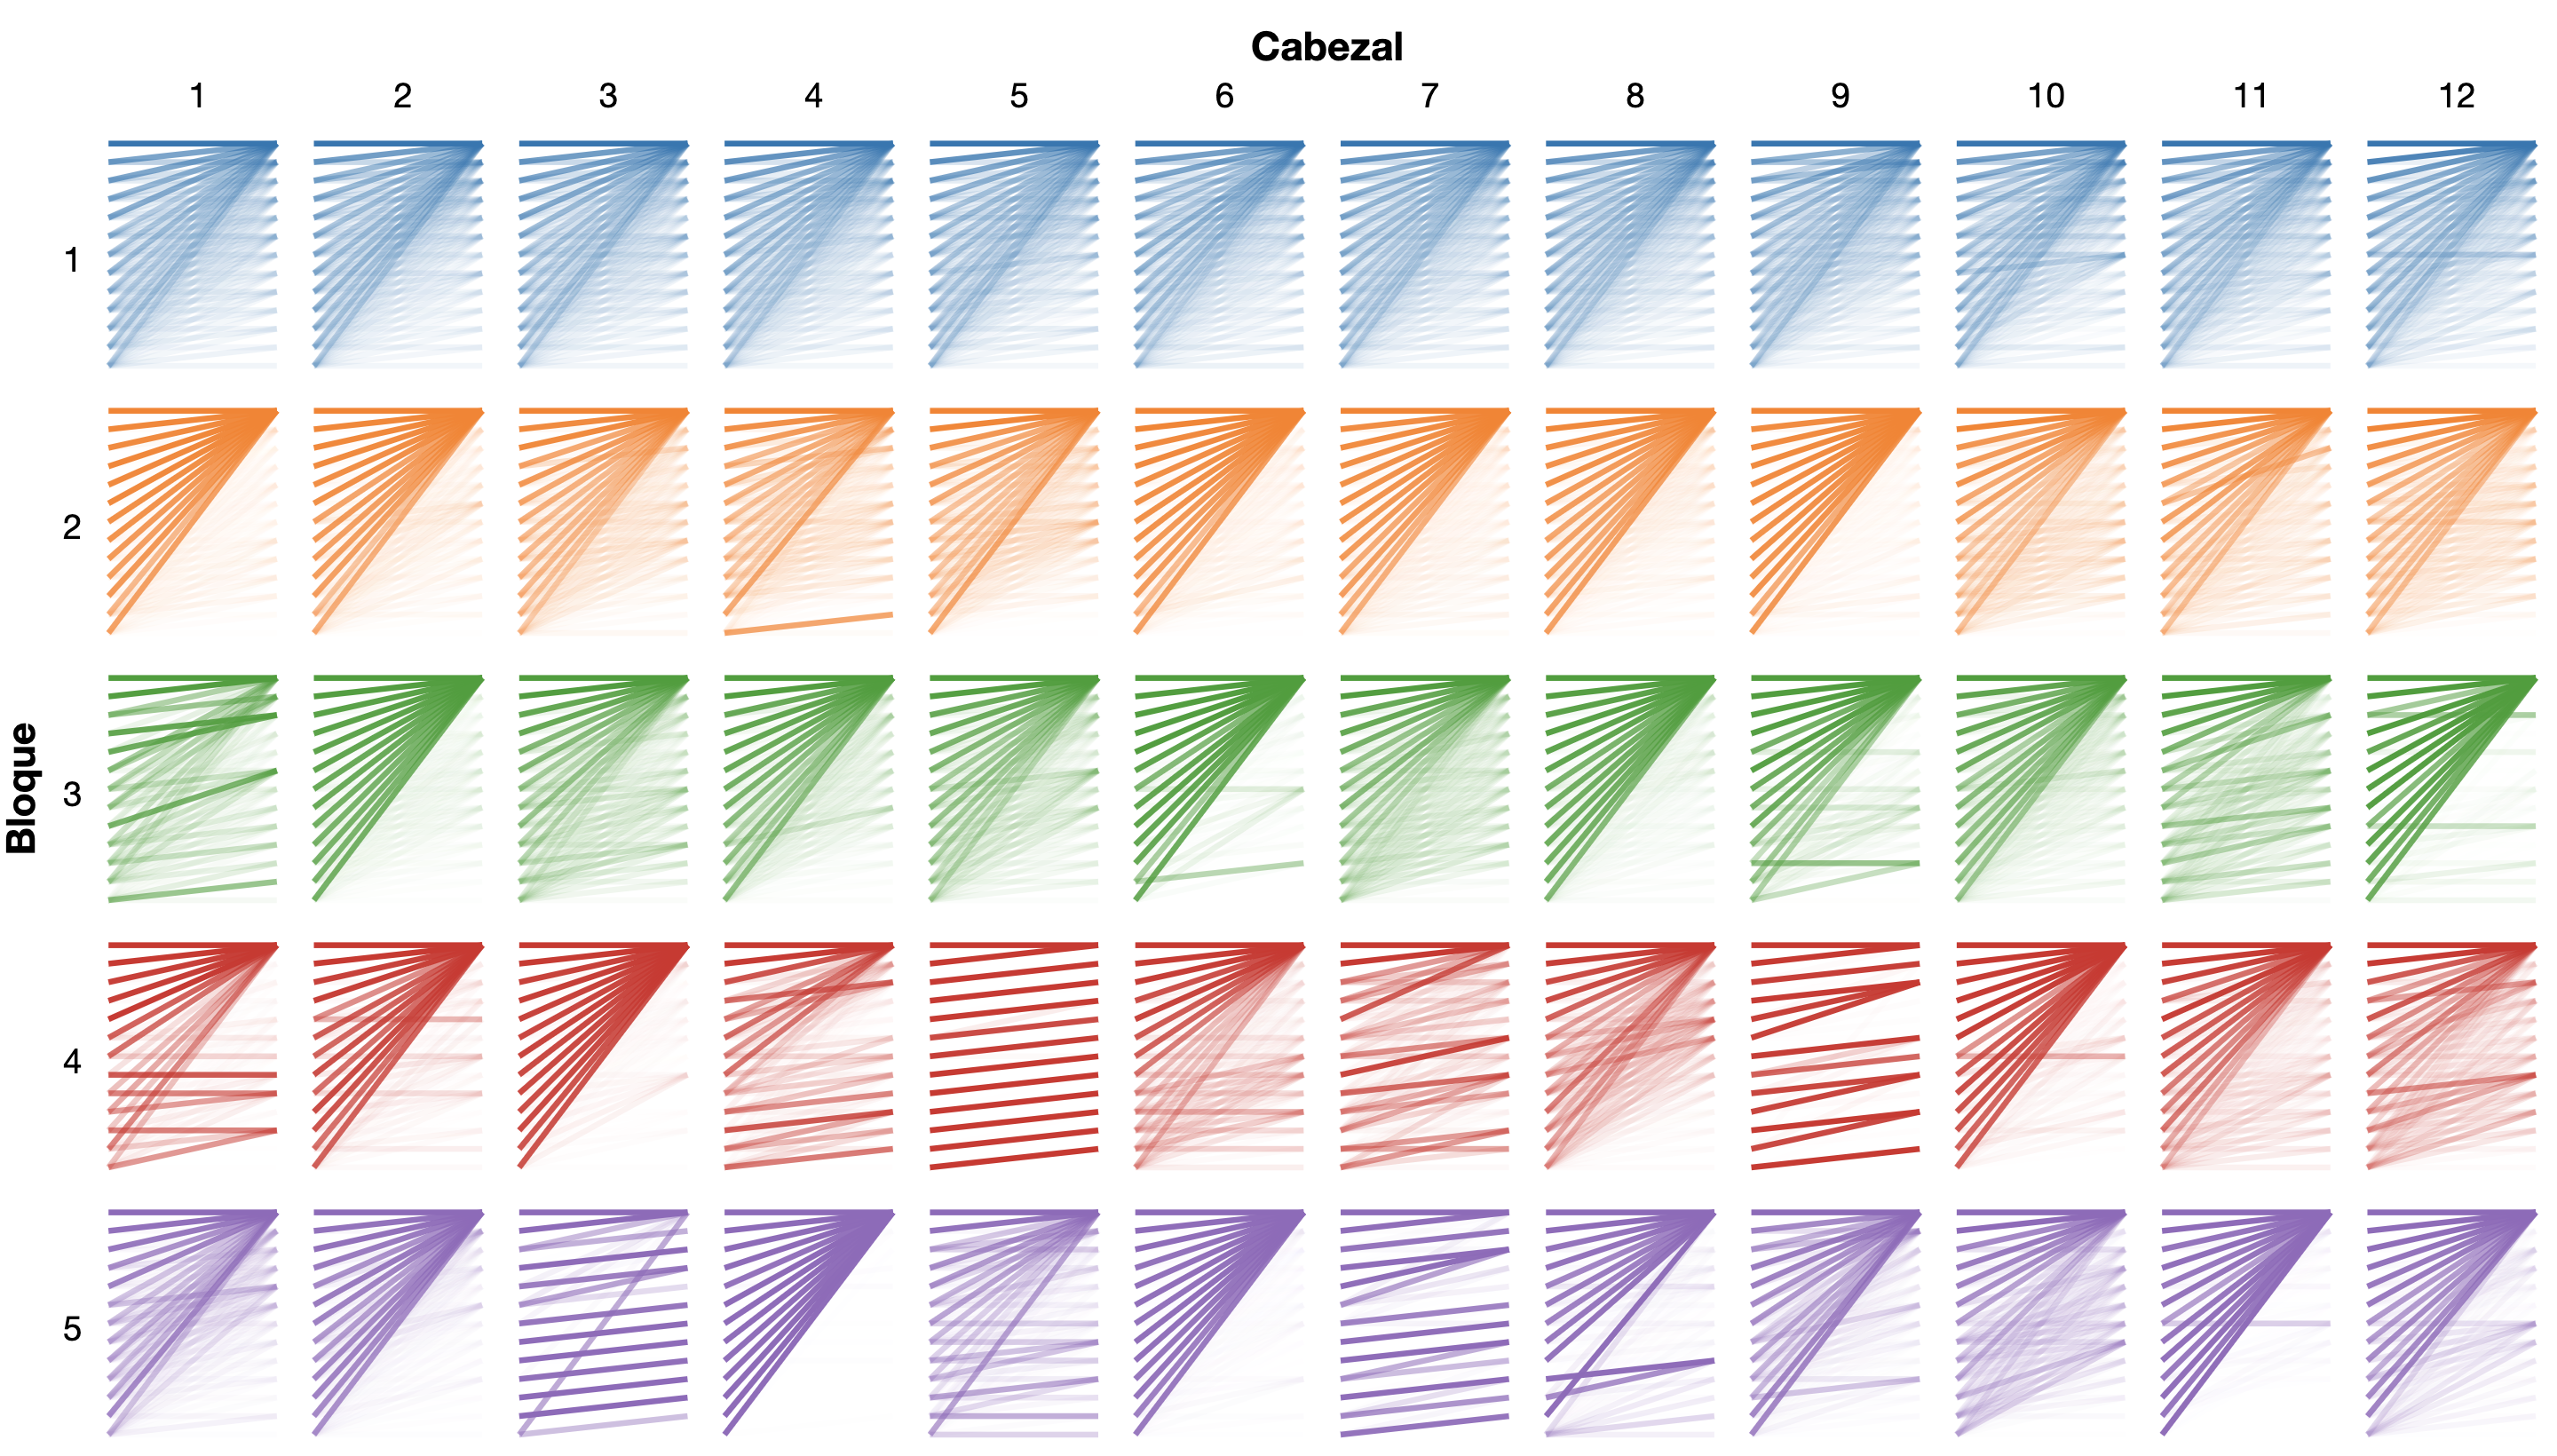
\includegraphics[width=\textwidth]{figures/chapter5/attention.png}
  \caption{Visualización de pesos de atención producidos por el modelo entrenado al procesar la secuencia (extraída literalmente del conjunto de entrenamiento) ``Buen remedio habeis hallado Para el mal de corazon'', que el \textit{tokenizador} entrenado codifica como ``Buen-remedio-hab-e-is-hallado-Para-el-mal-de-cora-zon''. }
  \label{fig:attention_visualizada}
\end{figure}

La \cref{fig:attention_visualizada} muestra la representación de los pesos de atención en los doce cabezales de atención presentes en los cinco primeros bloques del modelo GPT-2 entrenado. Como era de esperar, los distintos cabezales han aprendido comportamientos muy distintos aunque no es evidente cómo interpretar su función. La complejidad de extraer conclusiones sobre el comportamiento global de cada cabezal ha llevado a la investigación de métodos más sofisticados para visualizar la atención, el más significativo de los cuales (el despliegue de atención o \textit{vision rollout}) se presenta en el \cref{appendixB}.


